\documentclass{acm_proc_article-sp}
\usepackage[utf8]{inputenc}

\renewcommand{\paragraph}[1]{\vskip 6pt\noindent\textbf{#1 }}
\usepackage{hyperref}
\usepackage{graphicx}
\usepackage{url}

\providecommand{\tightlist}{%
  \setlength{\itemsep}{0pt}\setlength{\parskip}{0pt}}

\title{ShinyPET: A Predictive, Exploratory and Text RShiny Application
using Airbnb data}


% Add imagehandling

\numberofauthors{2}
\author{
\alignauthor Ang Su Yiin \\
        \affaddr{Singapore Management University}\\
       \email{\href{mailto:suyiin.ang.2020@mitb.smu.edu.sg}{\nolinkurl{suyiin.ang.2020@mitb.smu.edu.sg}}}
\and \alignauthor Joey Chua \\
        \affaddr{Singapore Management University}\\
       \email{\href{mailto:joey.chua.2020@mitb.smu.edu.sg}{\nolinkurl{joey.chua.2020@mitb.smu.edu.sg}}}
\and \alignauthor Kevin Gunawan Albindo \\
        \affaddr{Singapore Management University}\\
       \email{\href{mailto:kgalbindo.2019@mitb.smu.edu.sg}{\nolinkurl{kgalbindo.2019@mitb.smu.edu.sg}}}
\and }

\date{}

%Remove copyright shit
\permission{}
\conferenceinfo{} {}
\CopyrightYear{}
\crdata{}

% Pandoc syntax highlighting

% Pandoc citation processing
\newlength{\csllabelwidth}
\setlength{\csllabelwidth}{3em}
\newlength{\cslhangindent}
\setlength{\cslhangindent}{1.5em}
% for Pandoc 2.8 to 2.10.1
\newenvironment{cslreferences}%
  {}%
  {\par}
% For Pandoc 2.11+
\newenvironment{CSLReferences}[3] % #1 hanging-ident, #2 entry spacing
 {% don't indent paragraphs
  \setlength{\parindent}{0pt}
  % turn on hanging indent if param 1 is 1
  \ifodd #1 \everypar{\setlength{\hangindent}{\cslhangindent}}\ignorespaces\fi
  % set entry spacing
  \ifnum #2 > 0
  \setlength{\parskip}{#2\baselineskip}
  \fi
 }%
 {}
\usepackage{calc} % for calculating minipage widths
\newcommand{\CSLBlock}[1]{#1\hfill\break}
\newcommand{\CSLLeftMargin}[1]{\parbox[t]{\csllabelwidth}{#1}}
\newcommand{\CSLRightInline}[1]{\parbox[t]{\linewidth - \csllabelwidth}{#1}}
\newcommand{\CSLIndent}[1]{\hspace{\cslhangindent}#1}

\usepackage{graphicx}
\usepackage{float}
\usepackage{caption}
\captionsetup{skip=1pt}
\setlength{\textfloatsep}{2pt}
\setlength{\intextsep}{2pt}

\begin{document}
\maketitle

\begin{abstract}
The increasing availability of data has resulted in the increased demand
for data driven decisions. Although there is an extensive range of
commercial statistical tools, they are often subscription-based and
demand good technical knowledge to mine and draw insights from.
Therefore, it may not appeal to the average user. Using a collection of
R packages available, A R-Shiny application was developed for the
average user to perform exploratory and confirmatory analysis, text
mining and predictive analysis to formulate insights and make data based
decisions. We have used Airbnb data as our baseline for this project as
data generated is rich in information, consisting of structured,
unstructured (textual), and location data. This paper discusses the
application's design choices, use case and future works.
\end{abstract}

\emph{Keywords} - Airbnb, Exploratory Analysis, Confirmatory Analysis,
Text Mining, Predictive Analytics, Decision Making, R Shiny, Interactive
Data Visualisation.

\hypertarget{introduction}{%
\section{Introduction}\label{introduction}}

With the explosion of affordable data storage and processing
technologies, the demand for data-driven decision-making (DDDM) has
increased significantly. DDDM refers to the systematic analysis,
examination and integration of data to making strategic decisions,
rather than based on intuition or observation alone (Mandinach, 2012).
As well-published Geoffrey Moore opines, ``Without big data analytics,
companies are blind and deaf, wandering out onto the Web like deer on a
freeway.'' Research by (Yasmin, 2020) found that the use of data driven
decision making through analytics tools had a positive impact on firm
performance.

\hypertarget{motivation-of-the-application}{%
\section{Motivation of the
application}\label{motivation-of-the-application}}

This project was motivated by the increasing demand for data analytics
as well as the lack of open source tools for users to perform analytics
to undercover meaningful patterns from structured, textual and spatial
data.

Although, there is a wide range of commercial statistical and analytics
tools available, these tools are often subscription-based and require
technical knowledge to mine and draw insights from. Alternatively, open
source tools as such R allows for interactive data visualisations,
however users would require extensive programming background to generate
such insights.

As such, we have developed a free, user-friendly and interactive tool
with 3 modules : 1) Exploratory - allows users to identify interesting
patterns based on selected variables. Findings from the exploratory
module are augmented by a statistical test based on user's chosen
variables.\\
2) Text - users can be able to perform analysis on textual data to
generate more quantitative insights.\\
3) Predictive - enables users to prepare and build a variety of
prediction models without needing to have in-depth understanding of the
predictive models and its algorithms.

To achieve our objective, we have used Airbnb data as our baseline as
data generated is rich in information, including structured data such as
price and location, as well as unstructured data such as reviews and
listing descriptions. Thus, with our application, anyone and everyone
would be able to make data-based decisions effortlessly.

\hypertarget{review-and-critic-on-past-works}{%
\section{Review and critic on past
works}\label{review-and-critic-on-past-works}}

Lu, Y., Garcia, R., Hansen, B. et al.~(2017)
{[}\protect\hyperlink{ref-https:ux2fux2fdoi.orgux2f10.1111ux2fcgf.13210}{2}{]}
provides a comprehensive summary of research on Predictive Visual
Analytics. The paper discusses how visual analytics systems are
implemented to support predictive analytics process such as feature
selection, incremental learning, model comparison and result
exploration. The overall goal of visual analytics is to support
explanation in each step of predictive analytics exercise which is also
our motivation in developing this application.

Radiant package {[}\protect\hyperlink{ref-radiant2019}{3}{]}, an
open-source platform-independent browser-based interface for business
analytics in R, illustrate the robustness of Rshiny for web-based
application. Developed to promote quick and reproducible data analytics,
the package provides interactivity and flexibility in performing
predictive analysis. Most of the plots produced are of static nature and
can be enhanced by wrapping plotly around them. In addition, more recent
package such as visNetwork allows interactive tree visualisation which
will improve the assessment of decision tree model.

In R community, Tidymodels
{[}\protect\hyperlink{ref-tidymodels2020}{1}{]} has gained interest by
providing a framework for predictive modeling and machine learning. It
is aligned with the tidyverse principles which leads to a tidier and
consistent grammar in the predictive analytics process. Different models
offered in Radiant package are also available for implementation in
Tidymodels framework, which is why our application leverages Tidymodel
as the main framework to conduct predictive analytics on Airbnb data.

\hypertarget{design-framework}{%
\section{Design framework}\label{design-framework}}

Our target users for this application are the average users without any
programming or extensive statistical knowledge yet wants to make data
driven decisions. Thus, the design of Shiny PET is based on 3 main
principles - user-friendliness, interactivity and ease of understanding,
yet comprehensive enough for users to make data driven decisions. The
application's colour scheme is based on Airbnb's official colours -
Raush, Babu and Foggy (type of gray).

The application consist of three modules - Exploratory, Text and
Predictive.

\hypertarget{exploratory-module}{%
\subsection{Exploratory module}\label{exploratory-module}}

The exploratory module enables users to perform exploratory and
confirmatory analysis on selected variables to identify interesting
patterns. There are three sections in this module - observe, map and
confirm \& explore.

\hypertarget{observe-submodule}{%
\subsubsection{Observe submodule}\label{observe-submodule}}

As shown in Figure {[}1{]}, the Observe section provides a summary of
the data for users to quickly understand and form questions surrounding
the data. Hence, this section was designed mainly based on ease of
understanding principles.

\begin{figure}[H]

{\centering 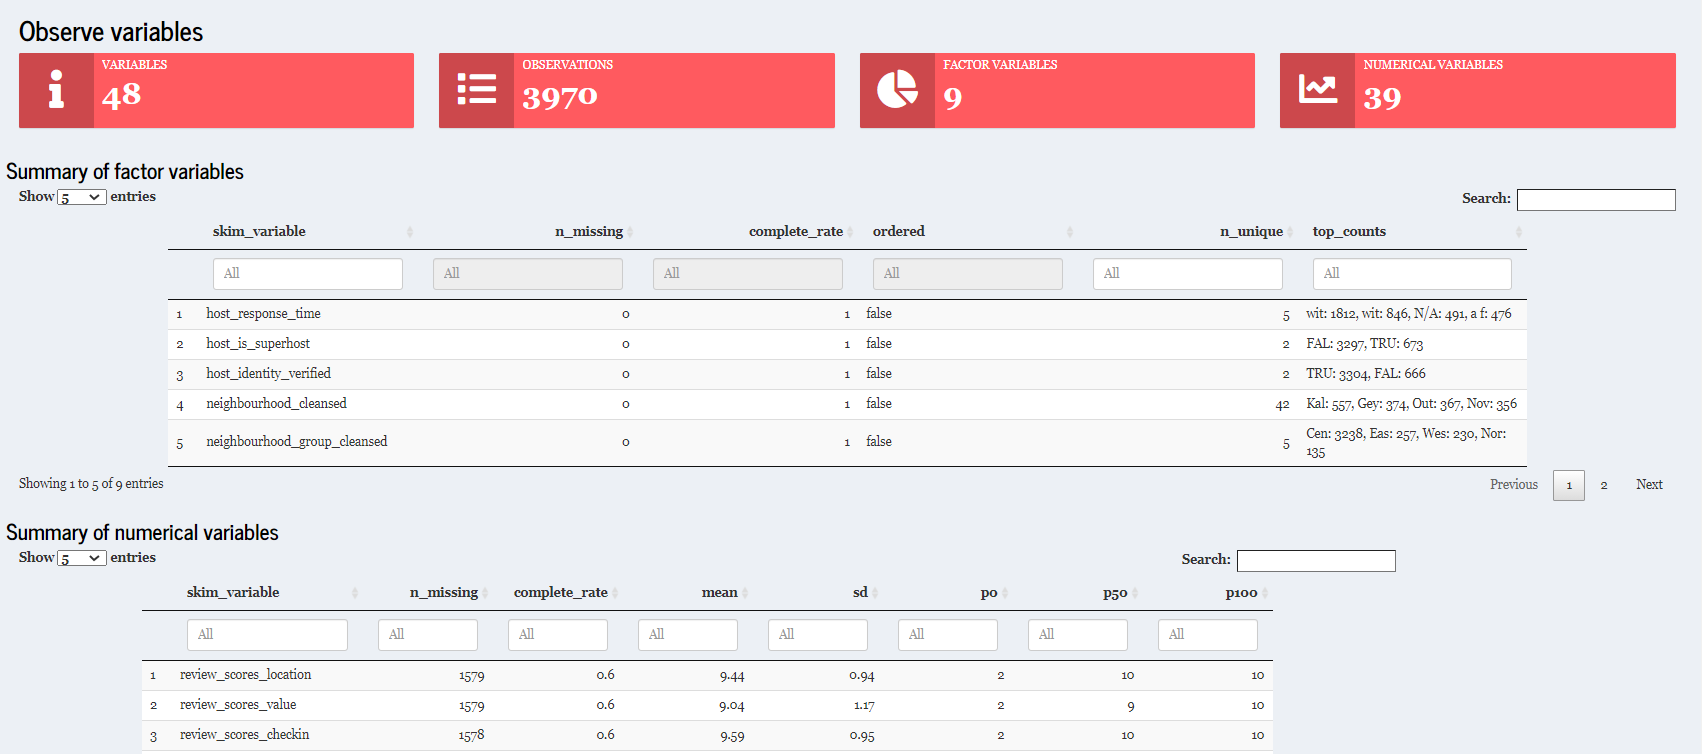
\includegraphics[width=1\linewidth]{images/design_observe} 

}

\caption{Interface and components of Observe section}\label{fig:unnamed-chunk-1}
\end{figure}

There are two main components - first is the top 4 boxes that provide an
overview of the data - number of variables, observations and data type.
The second component is the tables below shows the summary of each
variable by respective data type. The tables allow for some
interactivity - search boxes allows user to filter the data accordingly,
while the arrow icons next to the variables names allow users to sort
the data according to their needs.

\hypertarget{map-submodule}{%
\subsubsection{Map submodule}\label{map-submodule}}

\begin{figure}[H]

{\centering 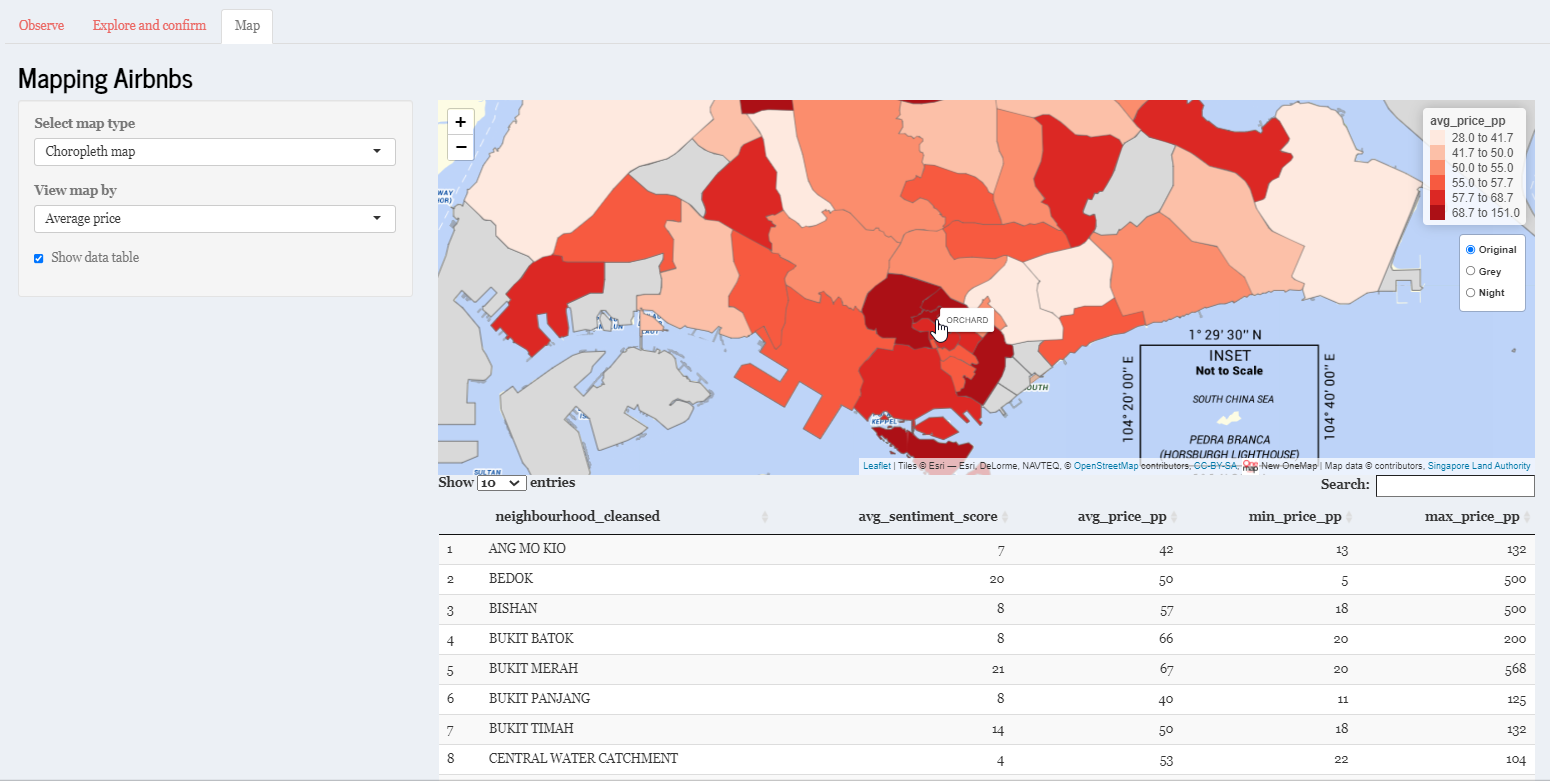
\includegraphics[width=1\linewidth]{images/design_map} 

}

\caption{Interface and components of Map section}\label{fig:unnamed-chunk-2}
\end{figure}

The Map section, Figure {[}2{]}, the Map section allows user to explore
the geographic patterns of Airbnb listings through thematic maps. Thus,
this section was designed based on the three principles stated above and
partially based on Shneiderman's interactive dynamics principle of
``overview, zoom and filter, then details on demand,'' save for the
`zoom and filter' portion as it was not applicable to this data.

As such, there are 2 main components of this submodule - the map which
provides a macro overview of the Airbnb listings by the selected
variable. The second component is the table, which provides details of
the map.

\hypertarget{map-submodule-1}{%
\subsubsection{Map submodule}\label{map-submodule-1}}

The Explore and Confirm section, figure {[}3{]}, enables user to explore
and perform inferential statistics based on their exploration and
questions generated from the previous two sections.

\begin{figure}[H]

{\centering 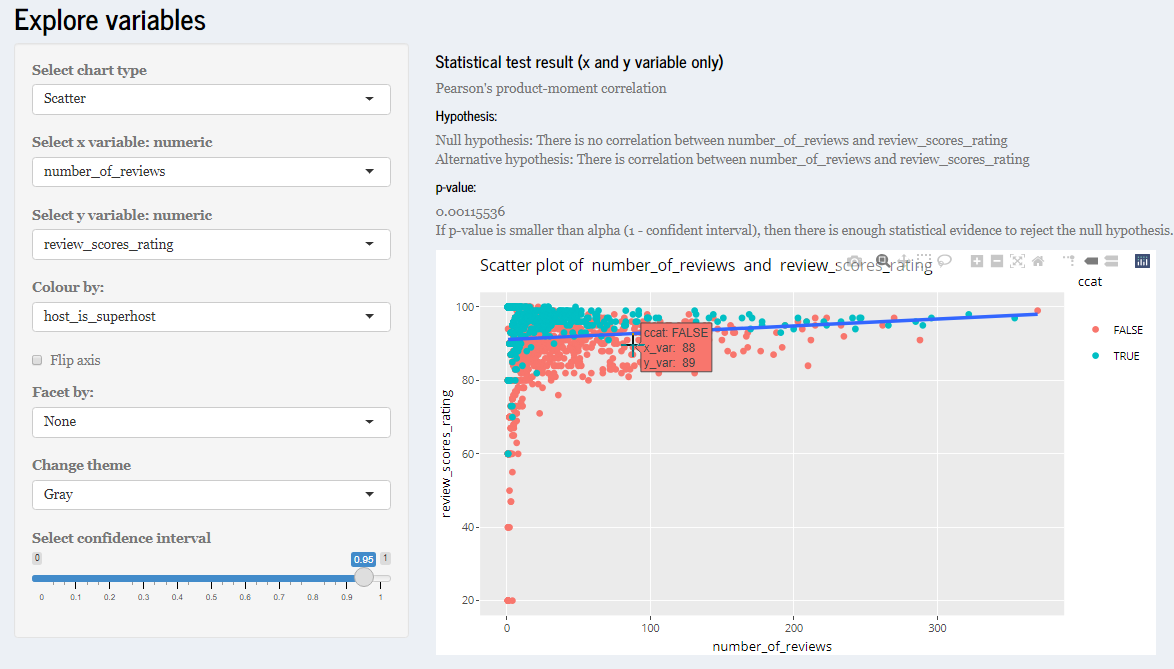
\includegraphics[width=1\linewidth]{images/design_explore1} 

}

\caption{Interface and components of Explore and Confirm section}\label{fig:unnamed-chunk-3}
\end{figure}

There are 3 main components - the selection input on the left, the
statistical results and the chart.

The selection input was designed to be interactive and user-friendly,
allowing users to customise charts based on the drop-down list provided.
The application provides for 4 types of chart namely: distribution,
mosaic, boxplot and scatter plot. In drop down menus will change
according to the selected chart type, for example, if the `Distribution'
chart was selected, only the x-variable drop-down input will be shown.

\begin{figure}[H]

{\centering 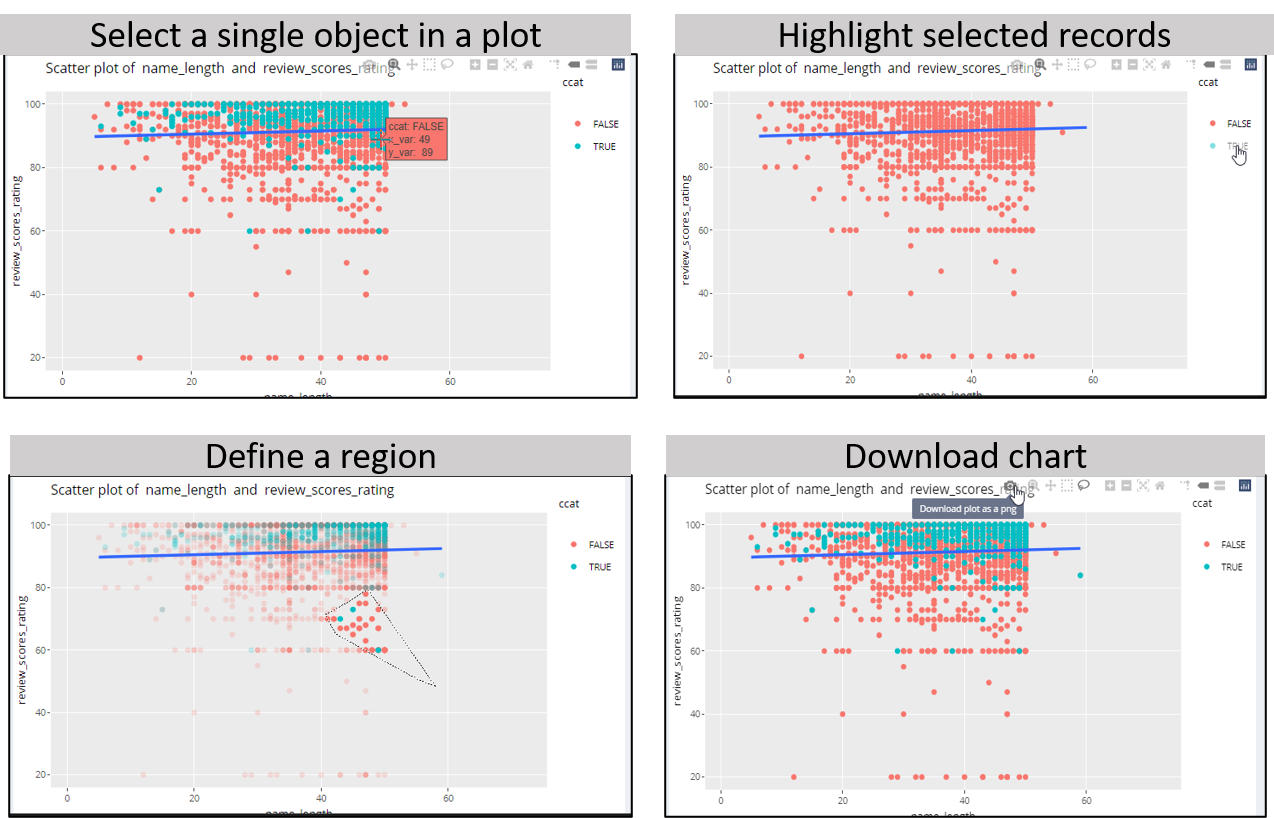
\includegraphics[width=1\linewidth]{images/design_explore2} 

}

\caption{Graph's manipulation function of the Explore and Confirm section}\label{fig:unnamed-chunk-4}
\end{figure}

The chart was designed according to Shneiderman's interactive dynamics
of highlight, filter or manipulate. This graph allows for users to
manipulate views by selecting a single object in a plot, highlighting
selected records and defining a region on the graph. Furthermore, the
plotted chart can be downloaded for users to communicate their findings.
See figure {[}4{]} for examples

Given that the application is tailored towards users that are not well
versed in statistics, the statistical test was designed to be easy to
understand, thus the test methods and results are automated based on the
selected variables. An interactive slider is provided for user to easily
adjust statistical test.

\hypertarget{text-module}{%
\subsection{Text module}\label{text-module}}

\hypertarget{predictive-module}{%
\subsection{Predictive module}\label{predictive-module}}

Our predictive module design framework follows Tidymodels framework for
data pre-processing, model training, tuning, and validation. On top of
that, feature selection are supported by other R packages such as
ggcorplot (for correlation matrix), ranger and Boruta (for feature
importance). The visualisation and interactivity are embedded in each
step of predictive analytics as explained below.

Data sampling - Selection of training-test split proportion provides
flexibility in deciding how to spend data budget on the model
development process. The distribution plot between training and test set
highlights any potential bias in the training data set.

\begin{figure}[H]

{\centering 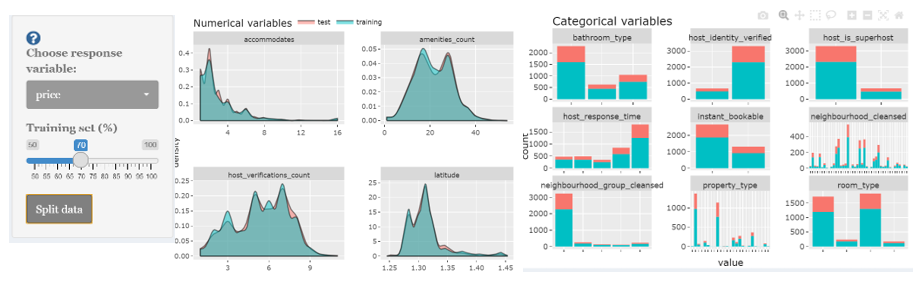
\includegraphics[width=1\linewidth]{images/datasplit} 

}

\caption{Data sampling and distribution plot}\label{fig:unnamed-chunk-5}
\end{figure}

Feature selection - Correlation matrix with customised correlation type
and p-value criteria, as well as variable importance allow assessment of
correlation among variables.

\begin{figure}[H]

{\centering 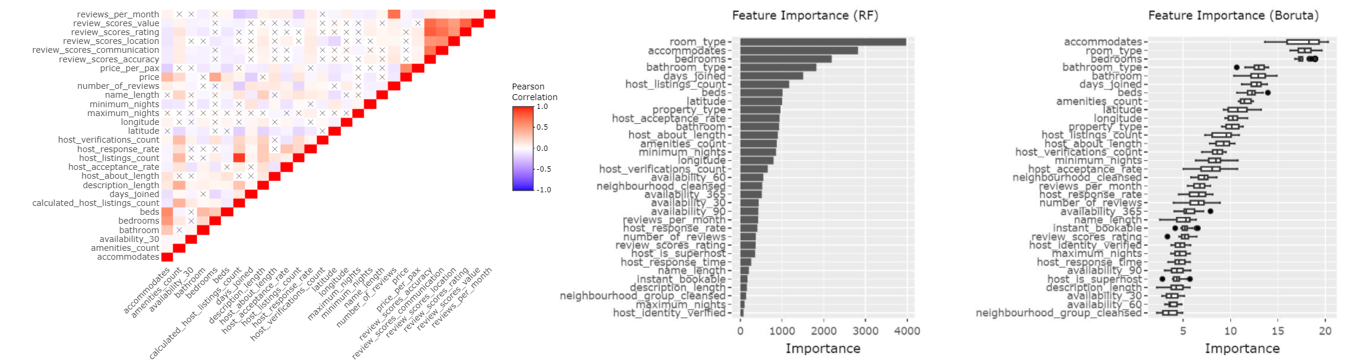
\includegraphics[width=1\linewidth]{images/featselect} 

}

\caption{Correlation matrix and variable importance}\label{fig:unnamed-chunk-6}
\end{figure}

Data transformation - Transformation steps from recipe package and plot
between pre and post processing step increases user awareness on what
transformation steps are performed and on which variables.

\begin{figure}[H]

{\centering 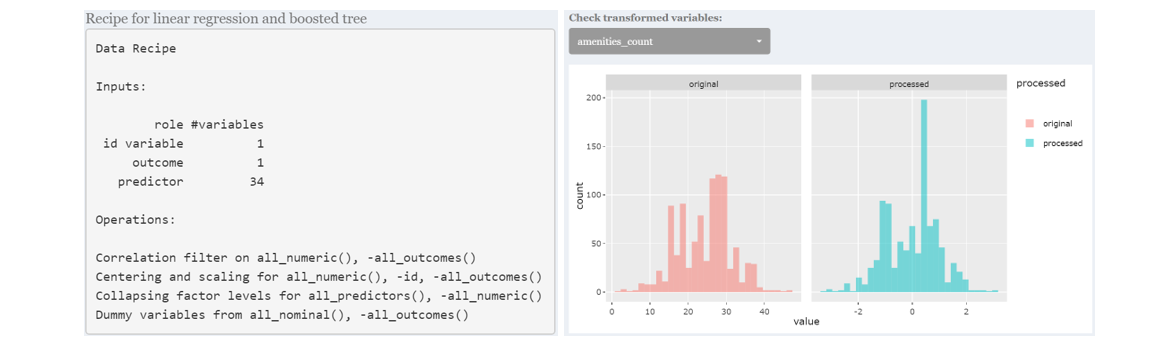
\includegraphics[width=1\linewidth]{images/recipetrf} 

}

\caption{Data transformation steps}\label{fig:unnamed-chunk-7}
\end{figure}

Model training - Coefficient estimate or decision tree information as
interactive plot to improve result evaluation.

\begin{figure}[H]

{\centering 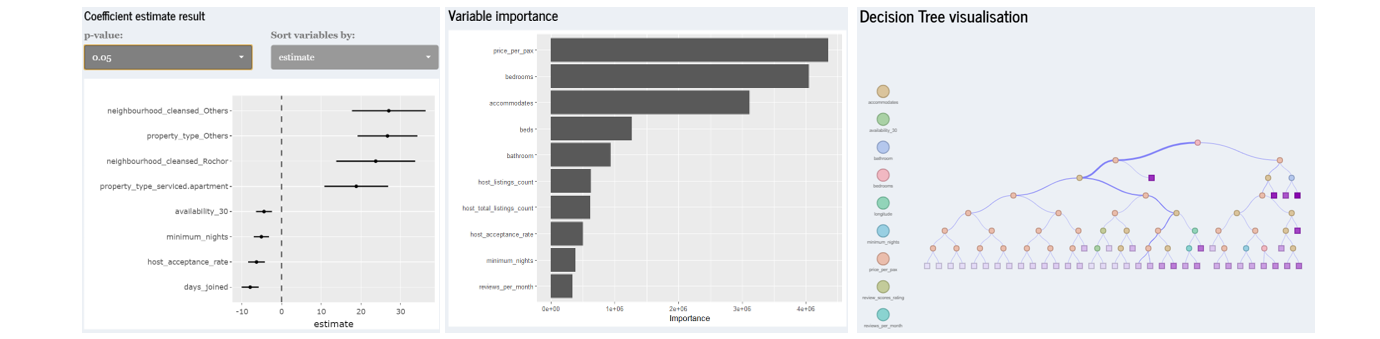
\includegraphics[width=1\linewidth]{images/mdltrn} 

}

\caption{Training result evaluation}\label{fig:unnamed-chunk-8}
\end{figure}

Model validation - Rsquare plot to visualise validation result along
with table of metric performance.

\begin{figure}[H]

{\centering 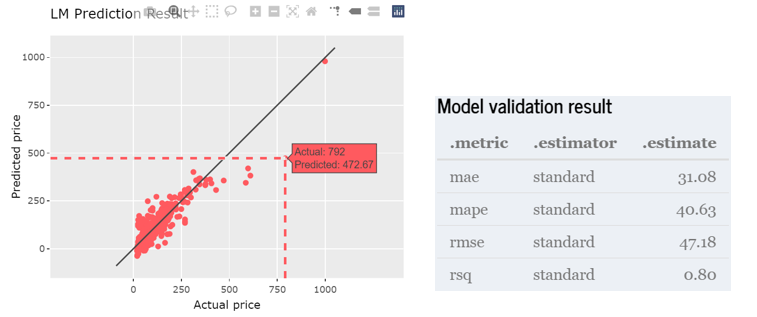
\includegraphics[width=1\linewidth]{images/mdleval} 

}

\caption{Validation result evaluation}\label{fig:unnamed-chunk-9}
\end{figure}

Prediction error assessment - Training set distribution plot is
overlapped with predicted values to allow further assessment on
prediction error.

\begin{figure}[H]

{\centering 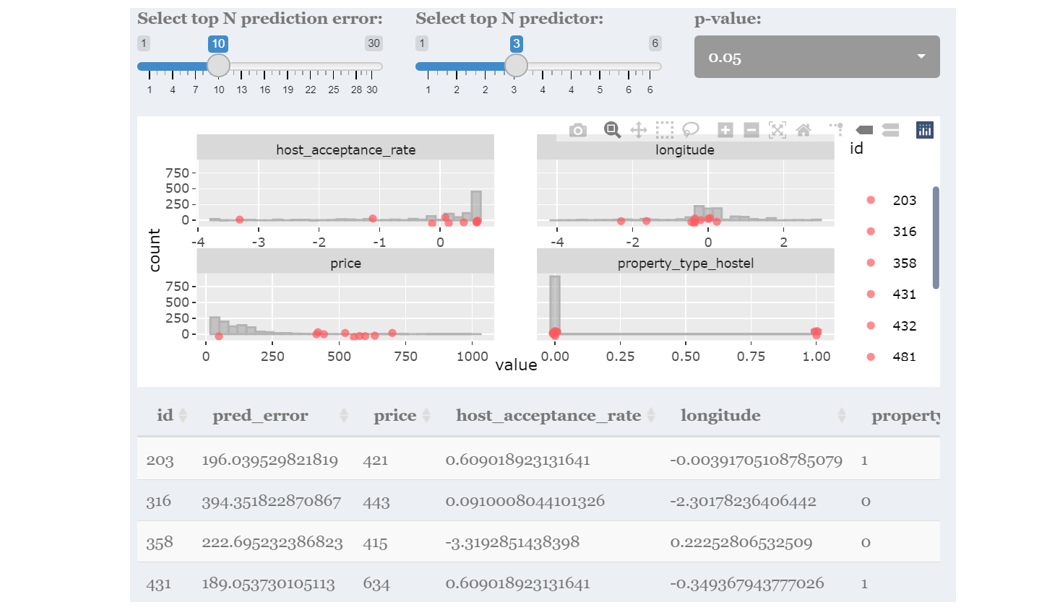
\includegraphics[width=1\linewidth]{images/prederror} 

}

\caption{Prediction error assessment}\label{fig:unnamed-chunk-10}
\end{figure}

Hyper-parameter tuning - Plot of model performance using different
hyper-parameters setting helps user to understand the change in
performance.

\begin{figure}[H]

{\centering 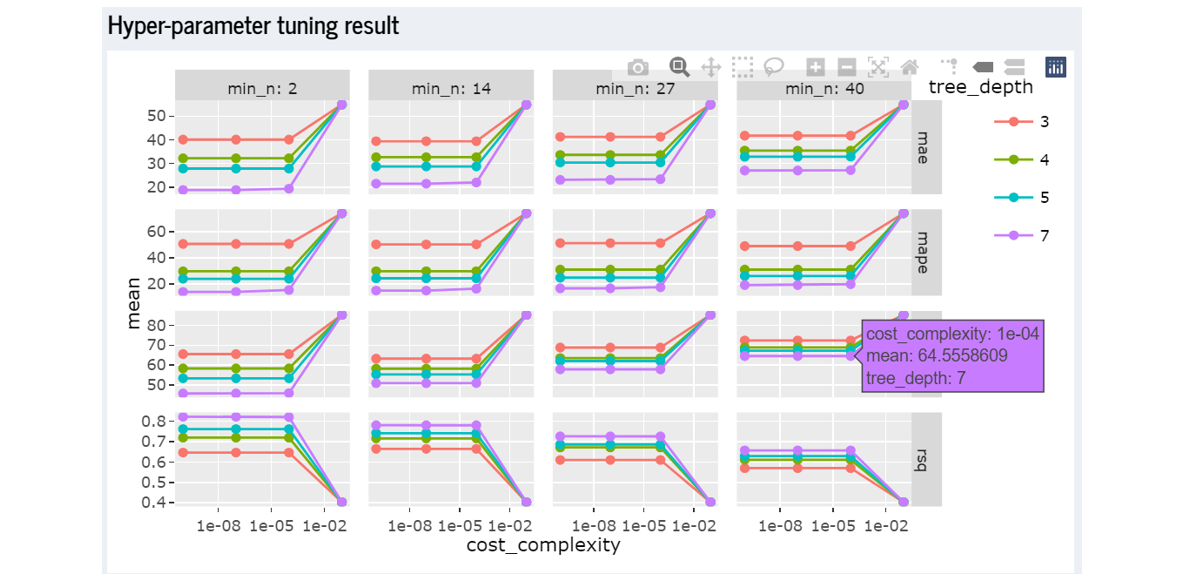
\includegraphics[width=1\linewidth]{images/hypartune} 

}

\caption{Hyper-parameter tuning result}\label{fig:unnamed-chunk-11}
\end{figure}

Model selection - Plot of performance metrics from different models to
support model selection process.

\begin{figure}[H]

{\centering 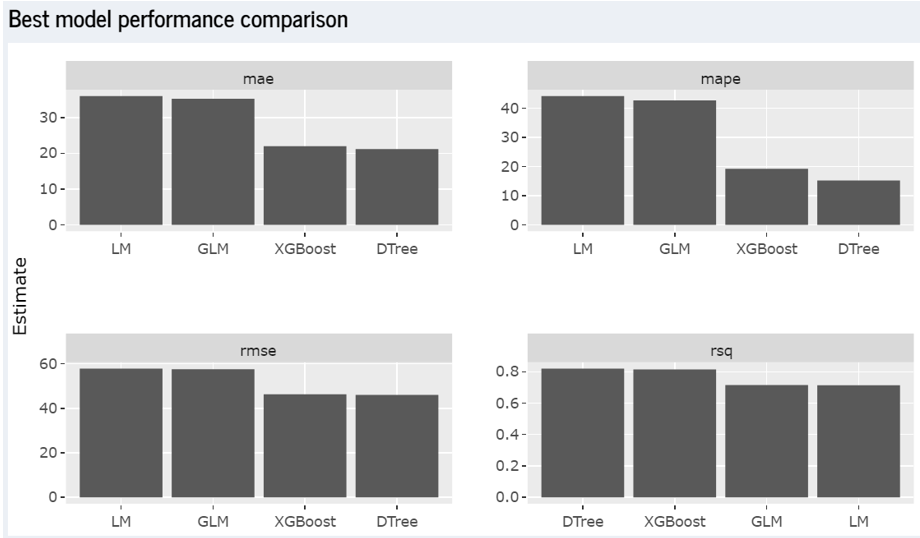
\includegraphics[width=1\linewidth]{images/mdlcompare} 

}

\caption{Models performance comparison}\label{fig:unnamed-chunk-12}
\end{figure}

\hypertarget{demonstration}{%
\section{Demonstration}\label{demonstration}}

\begin{itemize}
\tightlist
\item
  use case
\end{itemize}

\hypertarget{observing-correlation-among-variables}{%
\subsection{Observing correlation among
variables}\label{observing-correlation-among-variables}}

Data sets like Airbnb are rich with large numbers of variable. However,
multicolinearity among variables are known to affect predictive model
performance. Correlation matrix helps us to avoid such case by
highlighting variables with high correlation value. In our example
below, we observe correlations within rating score components, listing
availability period, and review components. With this information, we
can then select our variables more wisely.

\begin{figure}[H]

{\centering 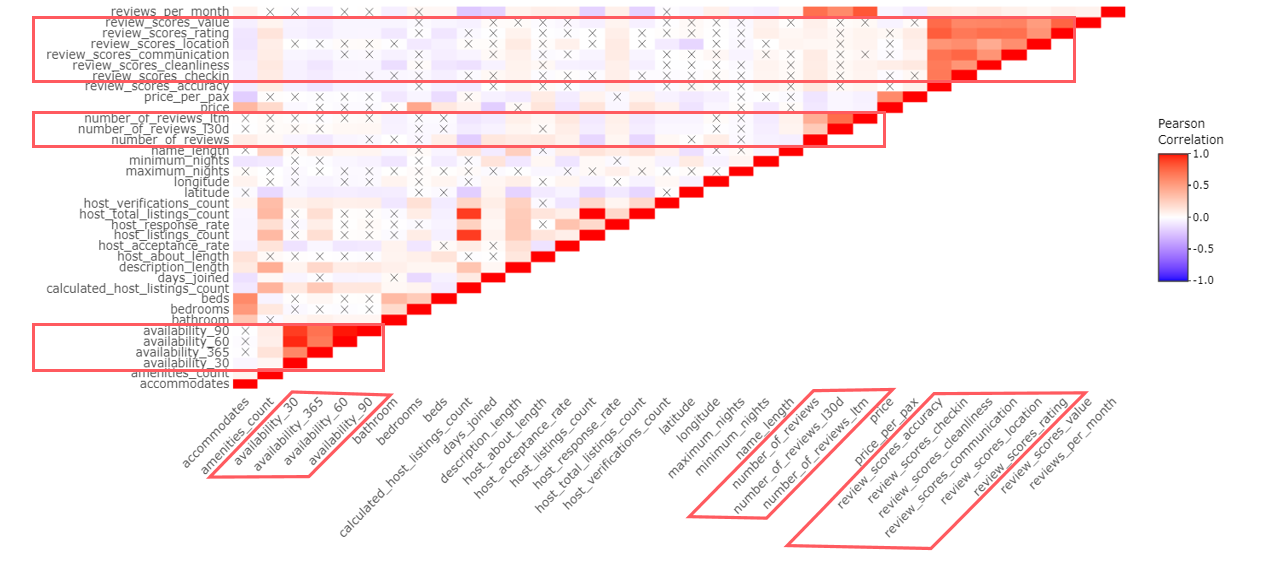
\includegraphics[width=1\linewidth]{images/corrcase} 

}

\caption{Correlation among variables}\label{fig:unnamed-chunk-13}
\end{figure}

\hypertarget{model-explanation}{%
\subsection{Model explanation}\label{model-explanation}}

In predicting listing price using linear model, the plot of coefficient
estimate helps to explain the trained model. In the example below, our
interface allows sorting of variables based on p-value score where
variables with lowest p-value is located on top. Property type which
falls under ``Others'' category (those with counts of less than 5\% in
the data set) has the lowest p-value score and positive estimate, which
may represent unique property type (e.g.~boat, campsite, chalet, villa)
where the listing price is above the average price of common property
type like apartment and condominium (as shown in the boxplot from
exploratory module). Amenities and beds are also in the top 5 predictor
where it correlates positively with listing price. However, the error
bar is wider for property type ``Others'' as compared to the amenities
and beds, representing more uncertainty in the estimate value.

\begin{figure}[H]

{\centering 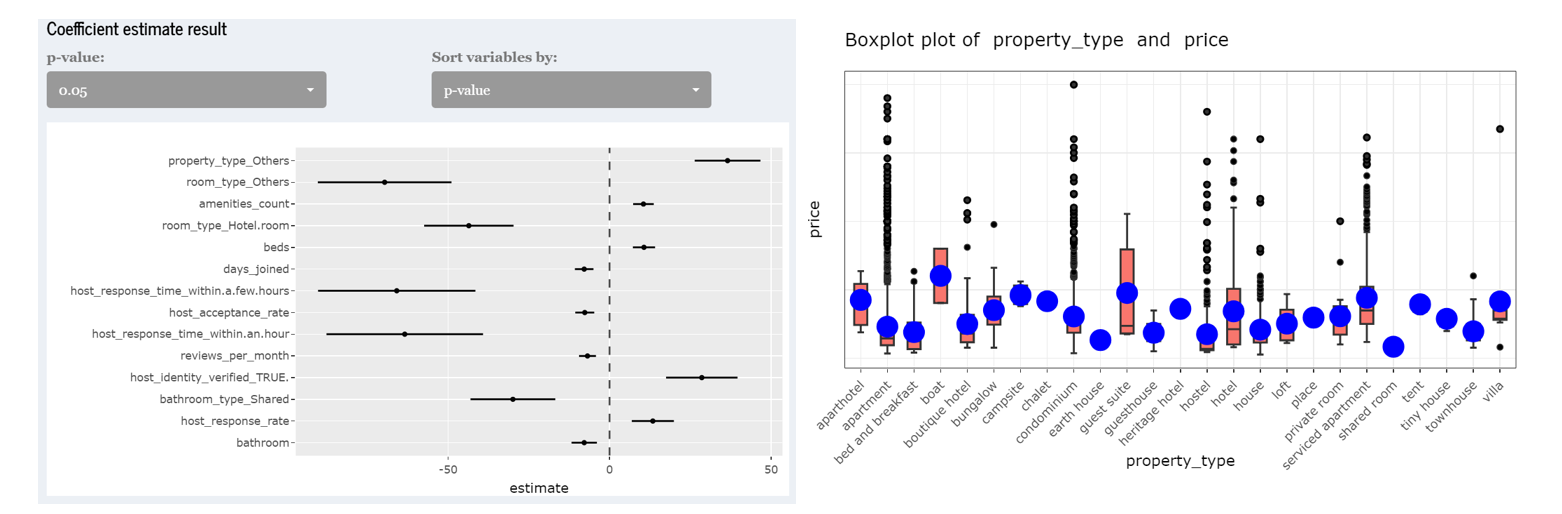
\includegraphics[width=1\linewidth]{images/LMcoeff} 

}

\caption{Coefficient estimate and boxplot from exploratory module}\label{fig:unnamed-chunk-14}
\end{figure}

\hypertarget{discussion}{%
\section{Discussion}\label{discussion}}

What has the audience learned from your work? What new insights or
practices has your system enabled? A full blown user study is not
expected, but informal observations of use that help evaluate your
system are encouraged.

\hypertarget{future-work}{%
\section{Future Work}\label{future-work}}

Shiny PET was built with Singapore's Airbnb dataset as a usecase for
using R Shiny to perform exploratory and confirmatory, text and
predictive analytics without users needing extensive programming or
statistical knowledge. Hence, the application could be further enhance
by including a data load and wrangling function to accommodate different
datasets.

Additionally, the current types of chart and statistical test are
limited with only 4 types of charts and parametric statistical test for
each chart type respectively. Other charts, such as violin and bar
charts, can be incorporated further. Additional hypothesis testing
methods can be included such as non-parametric test for median,
statistical test by pairs and others. The current application only
supports two types of map, other spatial maps such as kernel density map
and navigation map can be included.

The current predictive module is limited to 5 types of predictive model.
In future, more predictive models can be added to the list, such as
neural network to provide user with wider model selection. In terms of
hyper-parameter tuning, parameters can be made available for user input
to provide more flexibility in developing predictive model. In-depth
statistical analysis in model training such as residual analysis are
currently not available and this would be a good additional tool to
improve our application.

\hypertarget{acknowledgement}{%
\section{Acknowledgement}\label{acknowledgement}}

The authors wish to thank Professor Kam Tin Seong of Singapore
Management University for his extensive guidance and support during this
project.

\hypertarget{references}{%
\section*{References}\label{references}}
\addcontentsline{toc}{section}{References}

\hypertarget{refs}{}
\begin{CSLReferences}{0}{0}
\leavevmode\vadjust pre{\hypertarget{ref-tidymodels2020}{}}%
\CSLLeftMargin{{[}1{]} }
\CSLRightInline{Kuhn, M. and Wickham, H. 2020. \emph{Tidymodels: A
collection of packages for modeling and machine learning using tidyverse
principles.}}

\leavevmode\vadjust pre{\hypertarget{ref-https:ux2fux2fdoi.orgux2f10.1111ux2fcgf.13210}{}}%
\CSLLeftMargin{{[}2{]} }
\CSLRightInline{Lu, Y. et al. 2017. The state-of-the-art in predictive
visual analytics. \emph{Computer Graphics Forum}. 36, 3 (2017),
539--562.}

\leavevmode\vadjust pre{\hypertarget{ref-radiant2019}{}}%
\CSLLeftMargin{{[}3{]} }
\CSLRightInline{Nijs, V. 2019. \emph{Radiant -- business analytics using
r and shiny}.}

\end{CSLReferences}
\setlength{\parindent}{0in}

\end{document}
